\definecolor{C1}{RGB}{226, 43, 41}
\definecolor{C2}{RGB}{47, 96, 206}
\definecolor{C3}{RGB}{246, 175, 11} 


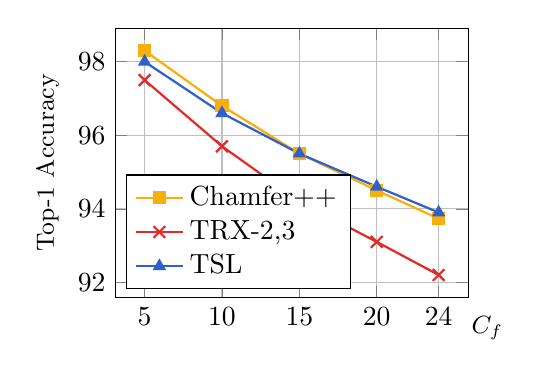
\begin{tikzpicture}
  \begin{axis}[
    width=0.5\linewidth,
    height=5cm, 
    xtick = {5,10,15,20,24},
	legend cell align={left},
	legend pos=south west,
    grid=both,
    ylabel={\small Top-1 Accuracy},
    xlabel={\small $C_f$},
    xlabel style={yshift=10pt, xshift=80pt,anchor=north east},
  ]

    \addplot [thick, color=C3, mark=square*,  mark size=2] coordinates {(5, 98.3) (10, 96.8) (15, 95.5) (20, 94.5) (24, 93.73)};   
    \addlegendentry{Chamfer++}  
	
    \addplot [thick, color=C1, mark=x,  mark size=3] coordinates {(5, 97.5) (10, 95.7) (15, 94.2) (20, 93.1) (24, 92.2)};      
    \addlegendentry{TRX-{2,3}} 
	
    \addplot [thick, color=C2, mark=triangle*,  mark size=2] coordinates {(5, 98) (10, 96.6) (15, 95.5) (20, 94.6) (24, 93.9)};      
    \addlegendentry{TSL} 


  \end{axis}
\end{tikzpicture}